\chapter*{Making concrete statements}

\ifnotes

    Learning outcomes:
    
    \begin{itemize}
        \item Explain the difference between \emph{concrete} and \emph{abstract} statements
        \item Describe why \emph{essential} details should be included and \emph{incidental} details should omitted 
    \end{itemize}

    This is a "trick" question:
    
    \begin{itemize}
        \item abstract statements are simple to spot, because they are meaningless
        \item statements can only be judged concrete in the context of the rule that they are being used to illustrate
    \end{itemize}
   
    There are only two abstract statements "Once upon a time" and "Some time ago". All the others may be sufficiently concrete for some context.
    
    An example is created to illustrate/explore the understanding of a rule. If the rule being illustrated is about some process timing out after 3 minutes, "3 minutes later" may be a sufficiently concrete statement. If the term "yesterday" is well defined within the team's ubiquitous language it may be just as concrete as "at 3:30pm on 2015-05-12".
\fi 

\ifcontent

    A \textbf{\textit{concrete}} statement is hard to misinterpret.  An \textbf{\textit{abstract}} statement is easy to misinterpret. 
    
    At your tables, arrange the following statements on the abstract/concrete axis below:
    
    \begin{enumerate}
        \item At 09:45
        \item Once upon a time
        \item It is precisely 11:00:00 p.m. Pacific Time
        \item Yesterday
        \item At 3:30 pm on 2015-05-12
        \item Some time ago
        \item On 3/2/2004
        \item In the morning
        \item At 11:45 a.m. on Thursday morning
        \item 3 minutes later
    \end{enumerate}
    
    \vfill
    
    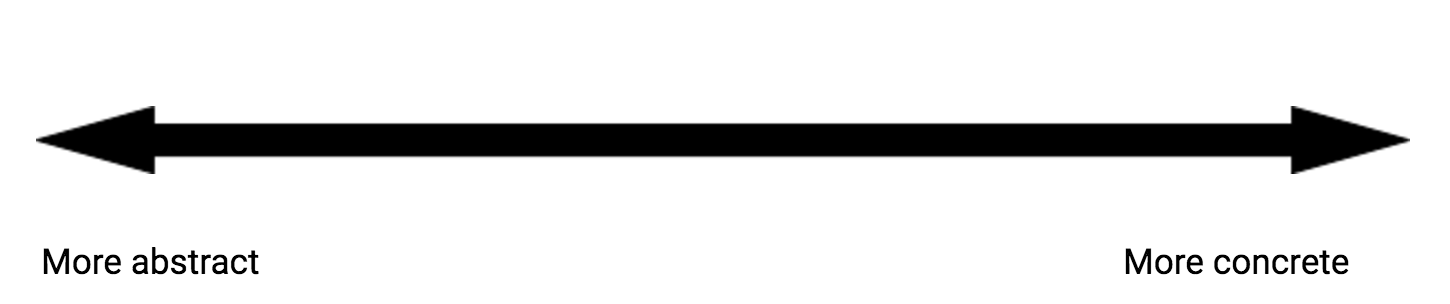
\includegraphics[width=\textwidth]{images/abstract-concrete-axis}
    
    \QandAbox{The concrete statements above have differing levels of detail. Is it always better to make your examples more detailed?}{2}

\fi